\section{Building the Translation Matrices} \label{sec:translation-matrices}

The core optimization of our FMM implementation is the precomputation of the translation matrices. These matrices are used to perform the various translations required by the FMM algorithm, such as \ac{P2M}, \ac{M2M}, \ac{M2L}, \ac{L2L}, and \ac{L2P}. We compute the matrices once upfront and store them in the \texttt{FMMNode} data structure for each node in the Octree. This allows us to avoid expensive redundant calculations during the FMM algorithm, significantly improving the computational efficiency of our implementation.

We group the discussion of the translation matrices by the stage of the tree traversal they are used in. This traversal process involves mathematically translating the source and destination points to the same coordinate system, which is then used to compute the translation matrices.

\begin{figure} [htpb] 
    \centering
    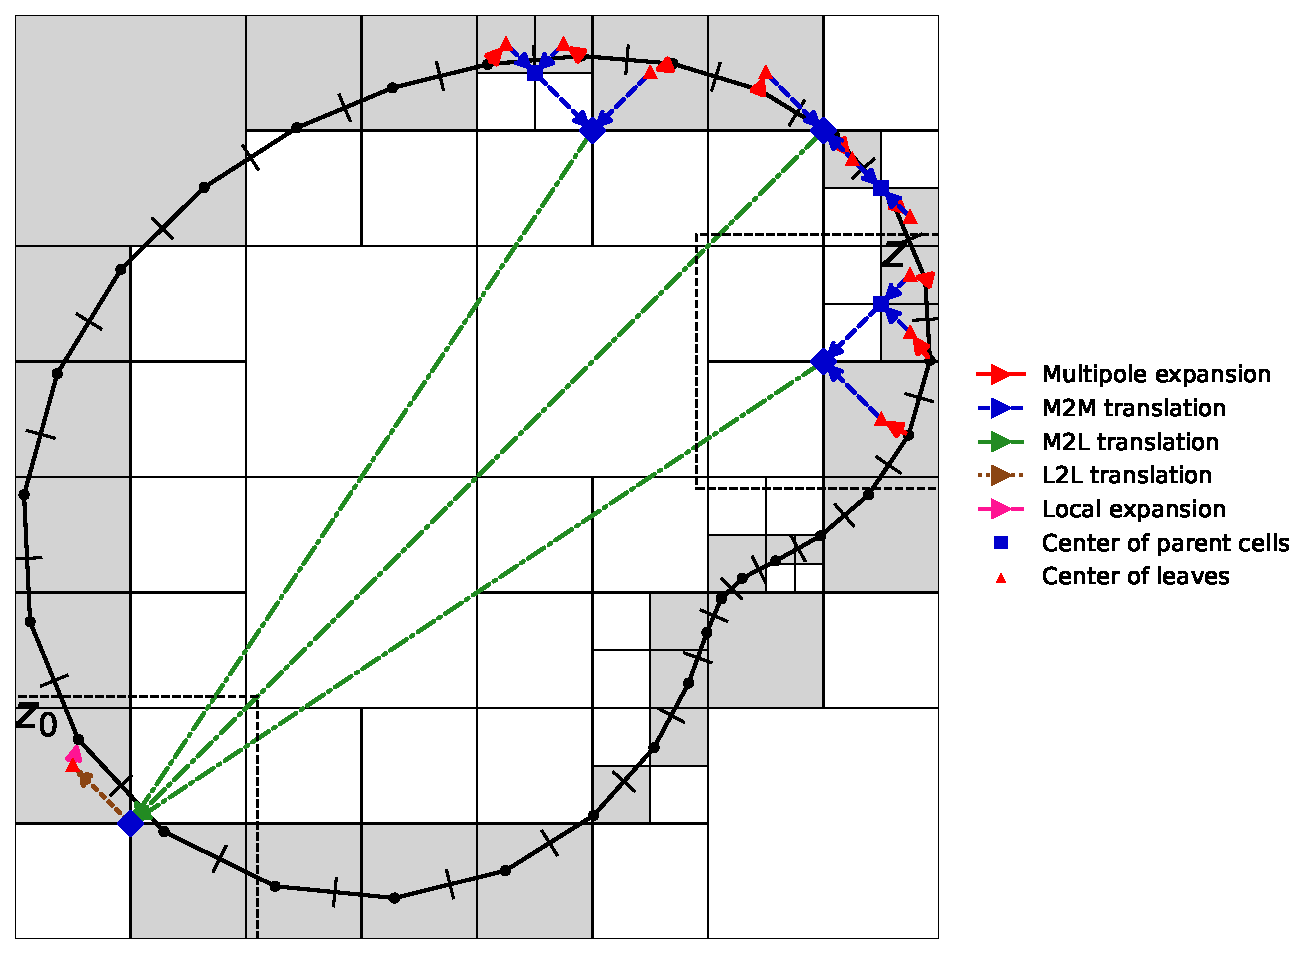
\includegraphics[width=0.8\textwidth]{figures/diagram_3_fmm_main.pdf} 
    \caption{A simplified representation of the FMM algorithm's main steps. We show somw of the far-field interactions and how they are computed. The greea arrows represent the \ac{M2L} translations, the blue arrows represent the \ac{M2M} translations, and the red arrows represent the Multipole Expansions. The brown arrows represent the \ac{L2L} translations, and the orange arrows represent the \ac{L2P} local expansoins. \cite{liufastmultipoleboundary2006}}
    \label{fig:fmm-interaction}
\end{figure}

\begin{figure}[htpb]
    \centering
    \begin{subfigure}{0.48\textwidth}
        \centering
        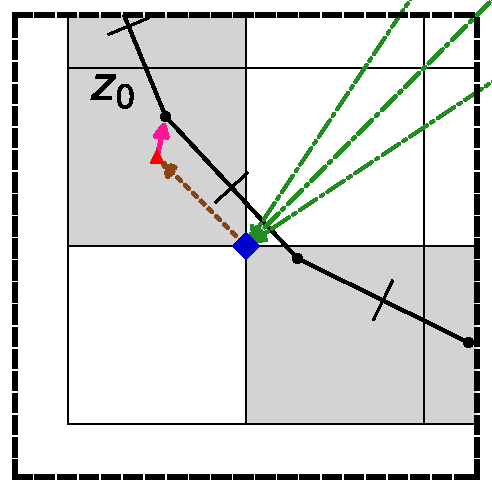
\includegraphics[width=\linewidth]{figures/diagram_4_fmm_target_zoom.pdf} 
        \caption{We can see how the incoming information from the \ac{M2L} interactionsis translated down to the leaf node, and the \ac{L2P} local expansion translates it onto the boundary element.}
        \label{fig:fmm-target-zoom}
    \end{subfigure}\hfill
    \begin{subfigure}{0.48\textwidth}
        \centering
        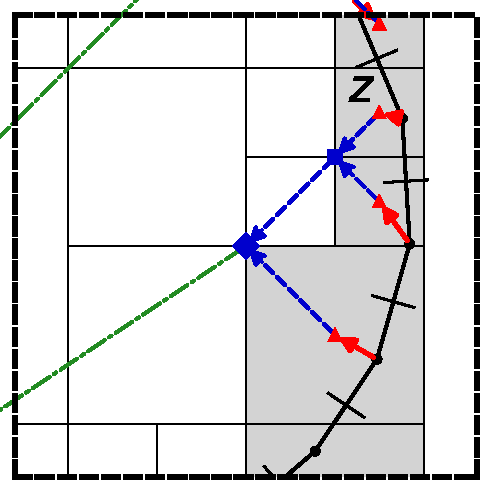
\includegraphics[width=\linewidth]{figures/diagram_5_fmm_source_zoom.pdf} 
        \caption{The upwards translation process, where the multipole expansion of the boundary element is translated up to the leaf node's center, and then up to the parent node's center with the \ac{M2M} translation, before being translated to the far-field node's center with the \ac{M2L} translation.}         
        \label{fig:fmm-source-zoom}
    \end{subfigure}
    \caption{Close up views of the translation process for the target and source nodes from \ref{fig:fmm-interaction} \cite{liufastmultipoleboundary2006}}
    \label{fig:translation-matrices-combined}
\end{figure}
